\section{Phonon-Mediated Attraction Between Electrons}

We've looked at some effects of electron-phonon interaction, but we have saved the most spectacular for last - that is superconductivity. Phonons can create attractive interactions between electrons, which can give rise to superconductivity - an interesting historical note is that this phenomenon was known experimentally for many decades before a good theory to describe it was discovered!

Recall the electron-electron interaction (photon exchange) in quantum electrodynamics - this leads to Coloumb repulsion. Analogously, we have an exchange of phonons between electrons in solids. However, this can give rise to attractive interactions - why? Photons travel at $c \gg v_{el}$, but phonons travel at the speed of sound $c_s \ll v_{el}$; it is a matter of relative velocities.

\subsection{Canonical Transformations}
We sketch a derivation of this based on the Frolich Hamiltonian. Our goal is to show that some attractive interaction is possible - we will not analyze this in great detail however. We are doing this primarily to introduce a new, very useful technique - known as \emph{canonical transformations}. We write:
\begin{equation}
    H = H_0 + H' = \sum_{\v{k}}\e_{\v{k}}c^\dag_{\v{k}}c_{\v{k}} + \sum_{\v{q}}\omega_{\v{q}}a^\dag_{\v{q}}a_{\v{q}} + M\sum_{\v{k}, \v{q}}c^{\dag}_{\v{k} + \v{q}}c_{\v{k}}(a^\dag_{-\v{q}} + a_{\v{q}}).
\end{equation}
From this we want to derive an effective ``electron-only'' Hamiltonian $H_{eff}$. Diagramatically, the process we consider is:

\begin{figure}[htbp]
    \centering
    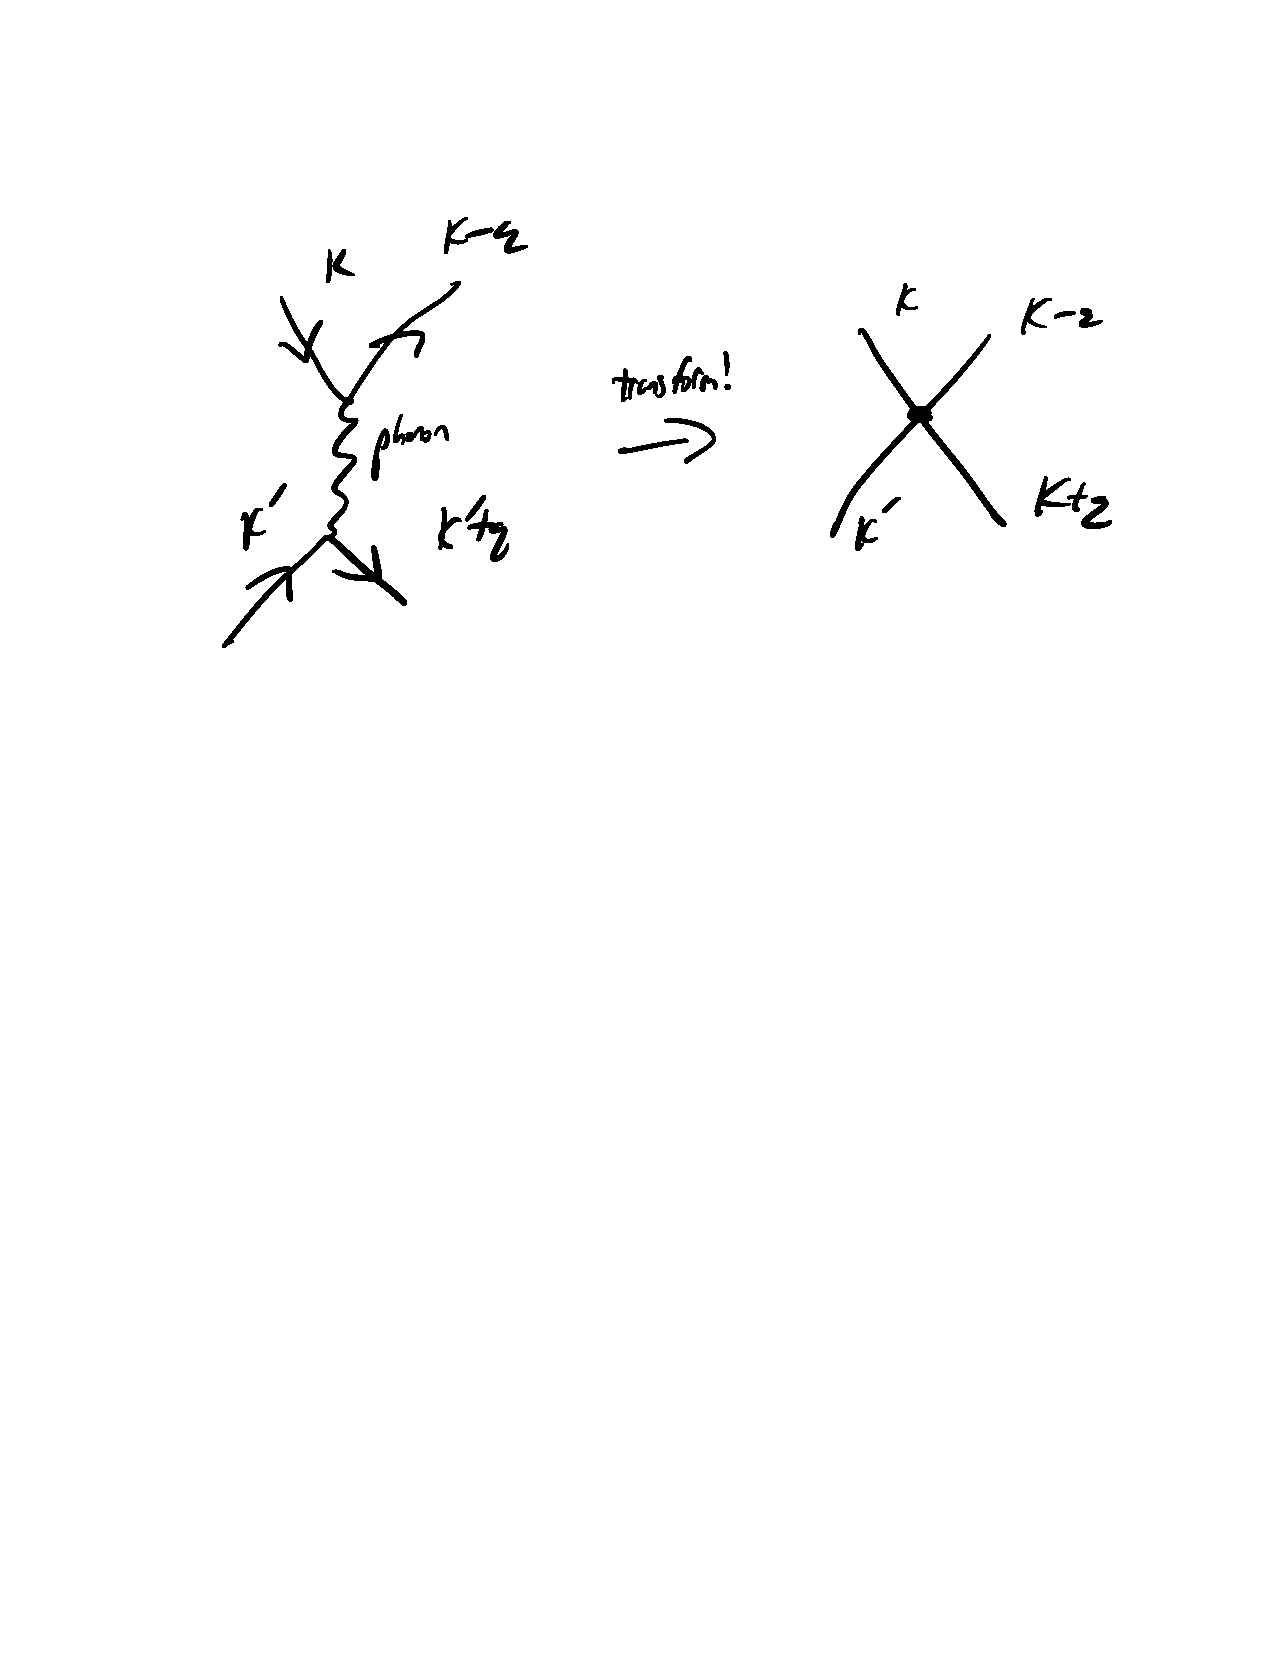
\includegraphics[scale=0.6]{Images/fig-electroninteractionfeynman.pdf}
    \caption{Feynman diagram for the electronic interaction via phonon exchange (left). Via a canonical transformation, we will recast this interaction into one that does not contain phonons (just electrons interacting - right).}
    \label{fig-electroninteractionfeynman}
\end{figure}

where we want to ignore the phonons and just consider an interaction between electrons (analogous to QED where one ignores the photon field). This is where canonical transformations will come in handy. We consider:
\begin{align*}
    H = H_0 + \lambda H'
\end{align*}
where $\lambda$ is some parameter. We transform it to:
\begin{equation}
    H \to \tilde{H} = e^{-S}He^{S} = H + [H, S] + \frac{1}{2}[[H, S], S] + \ldots
\end{equation}
usually in the literature, $S$ is anti-hermitian (hence the $i$s that you might expect are not written) but keep in mind that the above is a unitary transform. We have then expanded it using the Baker-Campbell-Hausdorf formula.

Now, we find an operator $S$ such that $\tilde{H}$ is independent of $\lambda$ to linear order. It may not be immediately obvious why this achieves what we want, but it will.

We then have:
\begin{equation}
    \tilde{H} = H_0 + \lambda H' + [H_0, S] + \lambda[H', S] + \ldots 
\end{equation}
We assume that $S$ must be linear in $\lambda$. So, $\lambda H' + [H_0, S]$ is linear in $\lambda$ and we demand it vanishes ($\lambda[H', S]$ is quadratic in $\lambda$, and so on for higher order terms)

We therefore find $S$ such that:
\begin{equation}
    [H_0, S] = -\lambda H'
\end{equation}
In some cases, if the operators are sufficiently simple one can find this directly. But there exists a way to find $S$ for an arbitrary situation - we proceed as follows. We adopt a basis $H_0\ket{\phi_m} = \e_m\ket{\phi_m}$. We then take matrix elements of both sides of the equation using these eigenstates:
\begin{align*}
    \bra{\phi_n}(H_0S - SH_0)\ket{\phi_m} = -\lambda \bra{\phi_n}H'\ket{\phi_m}
\end{align*}
Now, the trick is to act $H_0$ on the right and $H_0$ on the left, yielding the energy:
\begin{align*}
    (\e_n - \e_m)\bra{\phi_n}S\ket{\phi_m} = -\lambda \bra{\phi_n}H'\ket{\phi_m}
\end{align*}
So dividing by the energies, we can obtain arbitrary matrix elements of $S$ (note: it might seem like we run into trouble with this if we look at diagonal matrix elements - however we get around this by absorbing any diagonal perturbations into $H_0$, so the diagonal terms of $H'$ are zero)! I.e. we have the solution:
\begin{equation}
    \bra{\phi_n}S\ket{\phi_m} = \lambda\frac{\bra{\phi_n}S\ket{\phi_m}}{\e_m - \e_n}
\end{equation}
Finally, we have:
\begin{align*}
    \tilde{H} = H_0 + \lambda[H', S] + \frac{1}{2}[[H_0, S], S] + \frac{\lambda}{2}[[H', S], S]
\end{align*}
By assumption $[H_0, S] = -\lambda H'$, so $\lambda[H', S] + \frac{1}{2}[[H_0, S], S] = O(\lambda^2)$. But, $\frac{\lambda}{2}[[H', S], S] + \ldots O(\lambda^3)$. And so the result after combining everything is:
\begin{equation}
    \tilde{H} = H_0 + \frac{1}{2}\lambda [H',S] + O(\lambda^3).
\end{equation}
which achieves what we set out to do - we have found $S$ such that the transformed Hamiltonian is to leading order independent of $\lambda$! Next class, we apply this technique to the Frolich Hamiltonian. And when we evalute the $[H', S]$ term, we will see that it has no phonons, and corresponds to an attractive interaction.